\section{Use cases satisfaction: entities interactions}\label{use_cases_satisfaction}
This section will show how the entities introduced in the Architecture just presented actually cooperate with each other in order to satisfy the use cases previously discussed in \textit{section \ref{use_cases}}. 

\subsection{Contributor}
\begin{itemize}
    \item \textbf{Register}\\
    \begin{figure}[!ht]
        \centering
        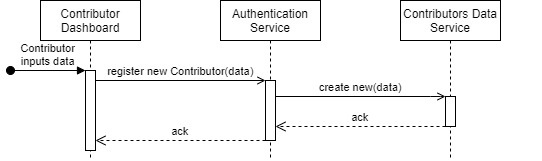
\includegraphics[scale=1]{document/chapters/chapter_6/images/use_cases_satisfaction_contributor_register.jpg}
        \caption{Contributor registration}
        \label{fig:use_cases_satisfaction_contributor_register}
    \end{figure}

    A Contributor registers to the Grid system creating an account using the Contributor Dashboard; once it has inputted the necessary data, the Dashboard will contact the Authentication with the dedicated API that, in turn, will contact the Contributors Data Service, actually completing the registration process.

    \item \textbf{Login}\\
    When a Contributor performs a Login, both in the Dashboard case and in the Contributing Endpoint, it gets a token that will be used for every subsequent operation for both authenticating the communication with other entities and, at the same time, provide some useful data that will be used by said entities.
    
    Since the token is a prerequisite for every further interaction it will be omitted for simplicity in the subsequent single use case satisfaction discussions. 
     
    \begin{itemize}
        \item \textbf{\textit{Login to a Dashboard}}\\
        \begin{figure}[!ht]
            \centering
            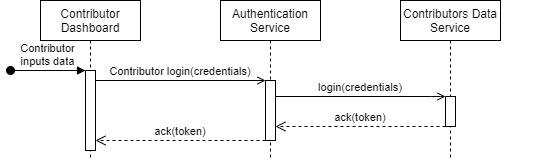
\includegraphics[scale=1]{document/chapters/chapter_6/images/use_cases_satisfaction_contributor_dashboard_login.jpg}
            \caption{Contributor Dashboard login}
            \label{fig:use_cases_satisfaction_contributor_dashboard_login}
        \end{figure}

        The login process performed by a Dashboard is very similar to the registration one, diverging only in the invocation of a different specific API.
        \vspace{4mm}

        \item \textbf{\textit{Login from any Contributing Endpoint able to Contribute}}\\
        \begin{figure}[!ht]
            \centering
            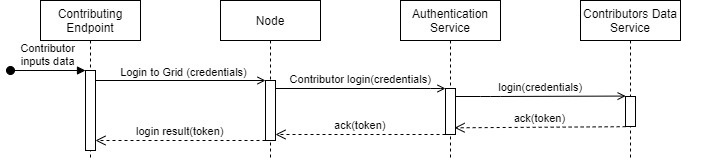
\includegraphics[scale=0.8]{document/chapters/chapter_6/images/use_cases_satisfaction_node_login.jpg}
            \caption{Node login}
            \label{fig:use_cases_satisfaction_node_login}
        \end{figure}

        Here, the Contributor Application is the one actually triggering the Login in its integrated Node; then, the Node's login differs from the Dashboard'one calling another dedicated API that also require to provide some additional info that will uniquely identify the device.
        
        The Customer only needs to make the active effort of registering its account; every Contributing Endpoint will be automatically added to its account if the credentials are correct and no matching device for its account is found.
        One important thing to notice is that the token does not exit the Node's scope.

    \end{itemize}

    \item \textbf{Passively Contribute offering a compatible device}\\
    When it comes to Contribution, the first step that actually needs to be performed is for a Node to connect to the Grid.
    \vspace{12mm}
    \begin{figure}[!ht]
        \centering
        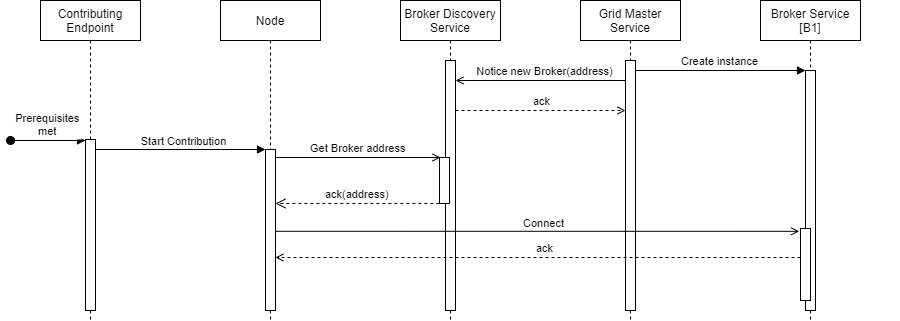
\includegraphics[width=\linewidth]{document/chapters/chapter_6/images/use_cases_satisfaction_node_grid_connection.jpg}
        \caption{Connection to the Grid}
        \label{fig:use_cases_satisfaction_node_grid_connection}
    \end{figure}
    \vspace{5mm}

    First, independently of the Node, the Grid Master Service creates an instance of a Broker Service (there is always at least one instance of such Cloud Service) and, upon creating a connection with it, saves its address; said address is also sent to the Broker Discovery Service that, consequently, will always locally know the addresses of the Broker Service's instances.

    The actual connection to the Grid is triggered automatically by the Contributing Endpoint once the prerequisites are met (an available internet connection is present, the device's battery is above a certain threshold, etc...). The Node will proceed to contact the Broker Discovery Service that (without needing to contact the Grid Master Service for every new Node request) then provides the address of the more geographically convenient Broker Service instance; with the information obtained, the Node completes it connection process contacting [B1]. 

    Now that the Node is connected to the Grid, the actual Contribution can happen. In order to have a clear understanding of the full picture, a Grid Service Invocation needs to be explained alongside the Node's Contribution.
    \vspace{10mm}

    \begin{figure}[!ht]
        \centering
        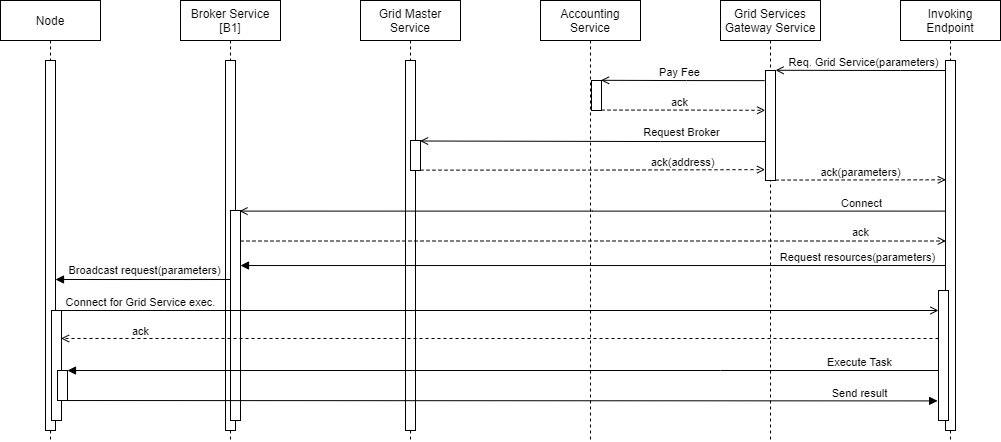
\includegraphics[width=\linewidth]{document/chapters/chapter_6/images/use_cases_satisfaction_node_contribution.jpg}
        \caption{Node Contribution}
        \label{fig:use_cases_satisfaction_node_contribution}
    \end{figure}

    The process starts with the Invoking Endpoint requesting a Grid Service to the Grid Services Gateway Service that, will first retrieve the Customer's payment method data (omitted in \textit{figure \ref{fig:use_cases_satisfaction_node_contribution}} for simplicity) and then contact the Accounting Service to pay the Fee required for the Grid Service Invocation; then, the Grid Services Gateway Service will contact the Grid Master Service in order to obtain the address of a Broker Service instance.

    The Invoking Endpoint, now having B1's address, contacts it and established a connection that, once performed, allows the Invoking Endpoint to request Resources. B1 broadcasts the request to all its Nodes, specifying the requirements needed for the Grid Service requested. The Nodes that are currently available, possess compatible Access Policies and do satisfy the requirements, take charge of the request and contact Invoking Endpoint and, if the Endpoint accepts it, a connection is created. Finally, the Invoking Endpoint is able to send Tasks that the Node will perform.

    The process describes an Invoking Endpoint to Node connection; when the connection needs to be established between Nodes, the process is very similar. First the Invoking Endpoint to Node connection is created; then, another Resource request will ask for a Contribution to the Nodes but the exchanged messages (containing the Master Node address) will specify that a Node to Node connection is required. Depending on the particular Grid Service then, the Master Node itself will provide the Tasks to its Slave Nodes.

    \begin{itemize}
        \item \textbf{\textit{Accumulate Rewards}}\\
        \begin{figure}[!ht]
            \centering
            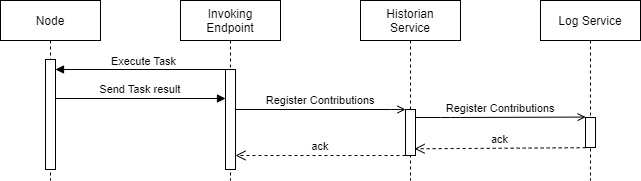
\includegraphics[scale=0.6]{document/chapters/chapter_6/images/use_cases_satisfaction_rewards_accumulation.jpg}
            \caption{Contributor's Rewards accumulation}
            \label{fig:use_cases_satisfaction_rewards_accumulation}
        \end{figure}

        Upon a Node's Contribution, the Invoking Endpoint groups Contribution info and sends them to the Historian Service that will then proceed to store them through the Log Service.

        \item \textbf{\textit{Manually start/stop Contribution from the Contributing Endpoint}}\\
        A Contributor can manually stop its Contributing Endpoint from performing further Contributions; this results in that particular Contributing Endpoint interrupting the connection (established in \textit{figure \ref{fig:use_cases_satisfaction_node_grid_connection}}) with a Broker Service instance.
        This action is performed by the Contributor's input in the running Contributing Endpoint that will simply invoke a Node's function instructing it to stop the connection and, consequently, never connecting again to the Grid until the Contributor allows it again.

        \item \textbf{\textit{Configure Access Policies to the Contributing Endpoint's Resources}}\\
        When a Node receives a broadcasted Contribution request by the Broker Instance which is connected to, in order to decide if taking charge of the request or not, a series of conditions are evaluated; one of such conditions is the compatibility with the local Access Policies configured for that particular Contributing Endpoint. 
        A Contributor, interacting with the Contributing Endpoint, can manually change the Access Policies that, from that moment, will be checked by the Node in its decision process. 

        \item \textbf{\textit{Check if Contributing Endpoints are currently Contributing}}\\
        The Node exposes functions that tell the current status regarding the Grid connection and if a Contribution to a Task is currently being performed; such information is displayed in the Contributing Endpoint's GUI.

    \end{itemize}
    \item \textbf{Manage Contribution data through a Dashboard}
    \begin{itemize}
        \item \textbf{\textit{Check past Contributions}}\\
        \begin{figure}[!ht]
            \centering
            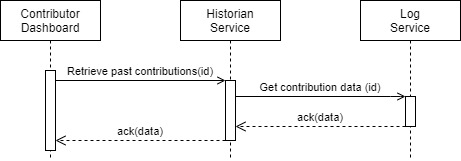
\includegraphics[scale=0.65]{document/chapters/chapter_6/images/use_cases_satisfaction_past_contributions_check.jpg}
            \caption{Contributor's past Contributions check}
            \label{fig:use_cases_satisfaction_past_contributions_check}
        \end{figure}

        The Contributor Dashboard contacts the Historian Service, asking for the past contributions linked to the Contributor's Contributing Endpoints; the Historian Service contacts the Log service where the data is stored (see \textit{figure \ref{fig:use_cases_satisfaction_rewards_accumulation}}). Finally, the information is retrieved and then shown in the Contributor Dashboard.

        \item \textbf{\textit{Check Rewards Balance}}\\
        \begin{figure}[!ht]
            \centering
            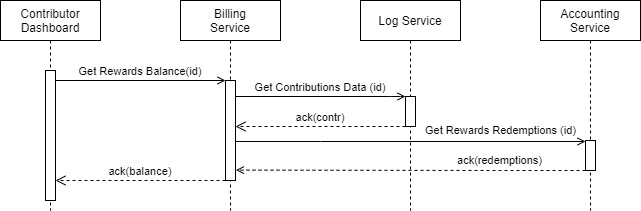
\includegraphics[scale=0.6]{document/chapters/chapter_6/images/use_cases_satisfaction_rewards_balance.jpg}
            \caption{Contributor's Rewards Balance check}
            \label{fig:use_cases_satisfaction_rewards_balance}
        \end{figure}

        The Contributor Data retrieves, through a communication with the Billing Service, its current Rewards Balance. In order to calculate the current balance, the Billing service contacts both the Log Service (to obtain the Contribution data) and the Accounting Service (to obtain past Rewards Redemptions). The Rewards Balance is calculated by the Billing Service by summing the monetary value of the Contributions and subtracting from it the total Rewards Redemption. 

        \item \textbf{\textit{Rewards Redemption}}\\
        \begin{figure}[!ht]
            \centering
            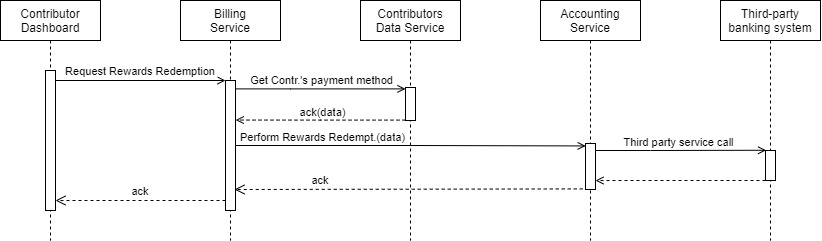
\includegraphics[width=\linewidth]{document/chapters/chapter_6/images/use_cases_satisfaction_rewards_redemption.jpg}
            \caption{Contributor's Rewards Redemption}
            \label{fig:use_cases_satisfaction_rewards_redemption}
        \end{figure}

        The Contributor Dashboard asks the Billing Service the execution of a Rewards Redemption. First the Contributors Data Service is contacted in order to retrieve the Contributor's payment method; then, the Log Service is contacted in order to retrieve the past Contributions data. Finally, the Accounting Service is interpellated, asking for the actual operation. The Accounting Service (that can access the past Rewards Redemptions on its own), performs the calculus of the Current Balance and, if the Balance is equal or higher than Rewards Threshold and, at the same time, compatible with the requested sum to redeem, the operation is finalized contacting a Third-party Banking System.

    \end{itemize}
\end{itemize}

\subsection{Customer}

\begin{itemize}
    \item \textbf{Register}\\
    The overall process is very similar to the one shown in \textit{figure \ref{fig:use_cases_satisfaction_contributor_register}}, interchanging the Contributor Dashboard with the Customer Dashboard and the Contributor Data Service with the Customer Data Service, respectively; while also the dedicated APIs are necessarily different, the registration process follows the same exact logical flow.

    \item \textbf{Login}\\
    \begin{itemize}
        \item \textbf{\textit{Login to a Dashboard}}\\
        \item \textbf{\textit{Authenticate for Grid Services Invocations}}\\
    \end{itemize}
    \item \textbf{Easily integrate the Invoking Endpoint in a Customer Custom Application}\\
    \begin{itemize}
        \item \textbf{\textit{Invoke Grid Services through any Device}}\\
        \item \textbf{\textit{Request MapReduce service}}\\
        \begin{itemize}
            \item \textit{Define MapReduce data source}\\
            \item \textit{Define Resource quantity to use}\\
            \item \textit{Define Map and Reduce functions}\\
        \end{itemize}
    \end{itemize}
    \item \textbf{Manage requested Grid Services data through a Dashboard}\\
    \begin{itemize}
        \item \textbf{\textit{Check Grid Services Invocations history}}\\
        \item \textbf{\textit{Check running Grid Services Invocations}}\\
        \item \textbf{\textit{Check past Grid Services Invocations Fees}}\\
        \item \textbf{\textit{Manage payment methods}}\\
    \end{itemize}
\end{itemize}